\section{Component View}
In this section, the individual components will be presented in terms of their functionalities, their role and the 
needed sub-parts, as well as how the sub-elements interface with one another within the overlaying component. Moreover, 
in this section it will be specified which of the considered sub-elements are in charge of interfacing with the other 
components of the system.

\begin{figure}[H]
  \centering
  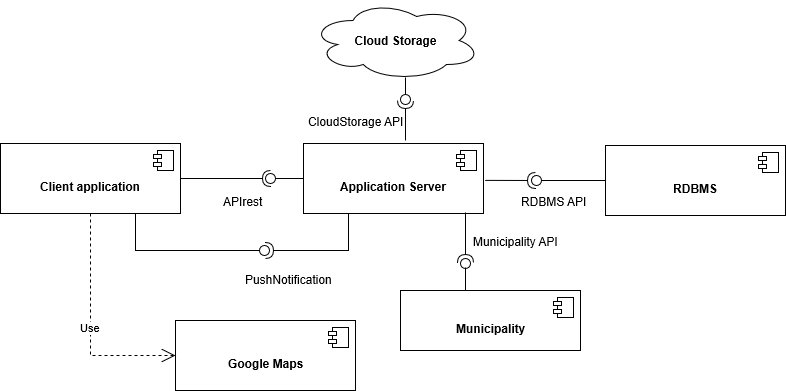
\includegraphics[origin=c,width=\textwidth]{DD_Images/ComponentView/componentView.jpg}
  \caption{\textit{Component View of the application}}
\end{figure}

\subsection{Database}
The database layer must include a DBMS component, in order to manage operations like selection, insertion, update or deletion.
The DBMS must guarantee the correct functioning of 
concurrent transactions and the ACID properties. As the application doesn’t require a more complex structure than the 
one provided by the relational data structure, the database has to be a RDBMS. The data layer will be exclusively 
accessible through the Application Server via a dedicated interface. Besides, the Application Server must provide a 
persistent unit to handle dynamic behavior of all the contained application data. 
\newline The system also provides an external Cloud Storage in order to memorize the pictures sent by the users that 
notify a violation. There is a dedicated service for this task because the amount of pictures that the application will
store will grow very fast. After saving pictures in the Cloud Storage, there is a unique identifier for every memorized data.
\newline Sensible data, fundamentally passwords, have to be hashed properly and salted before being stored. 
The users will be granted access only after verification of correct and valid credentials.
\newline Persistence and integrity are granted, as well as isolation in concurrent transactions and atomicity, all ACID properties 
are satisfied.

\begin{figure}[H]
  \centering
  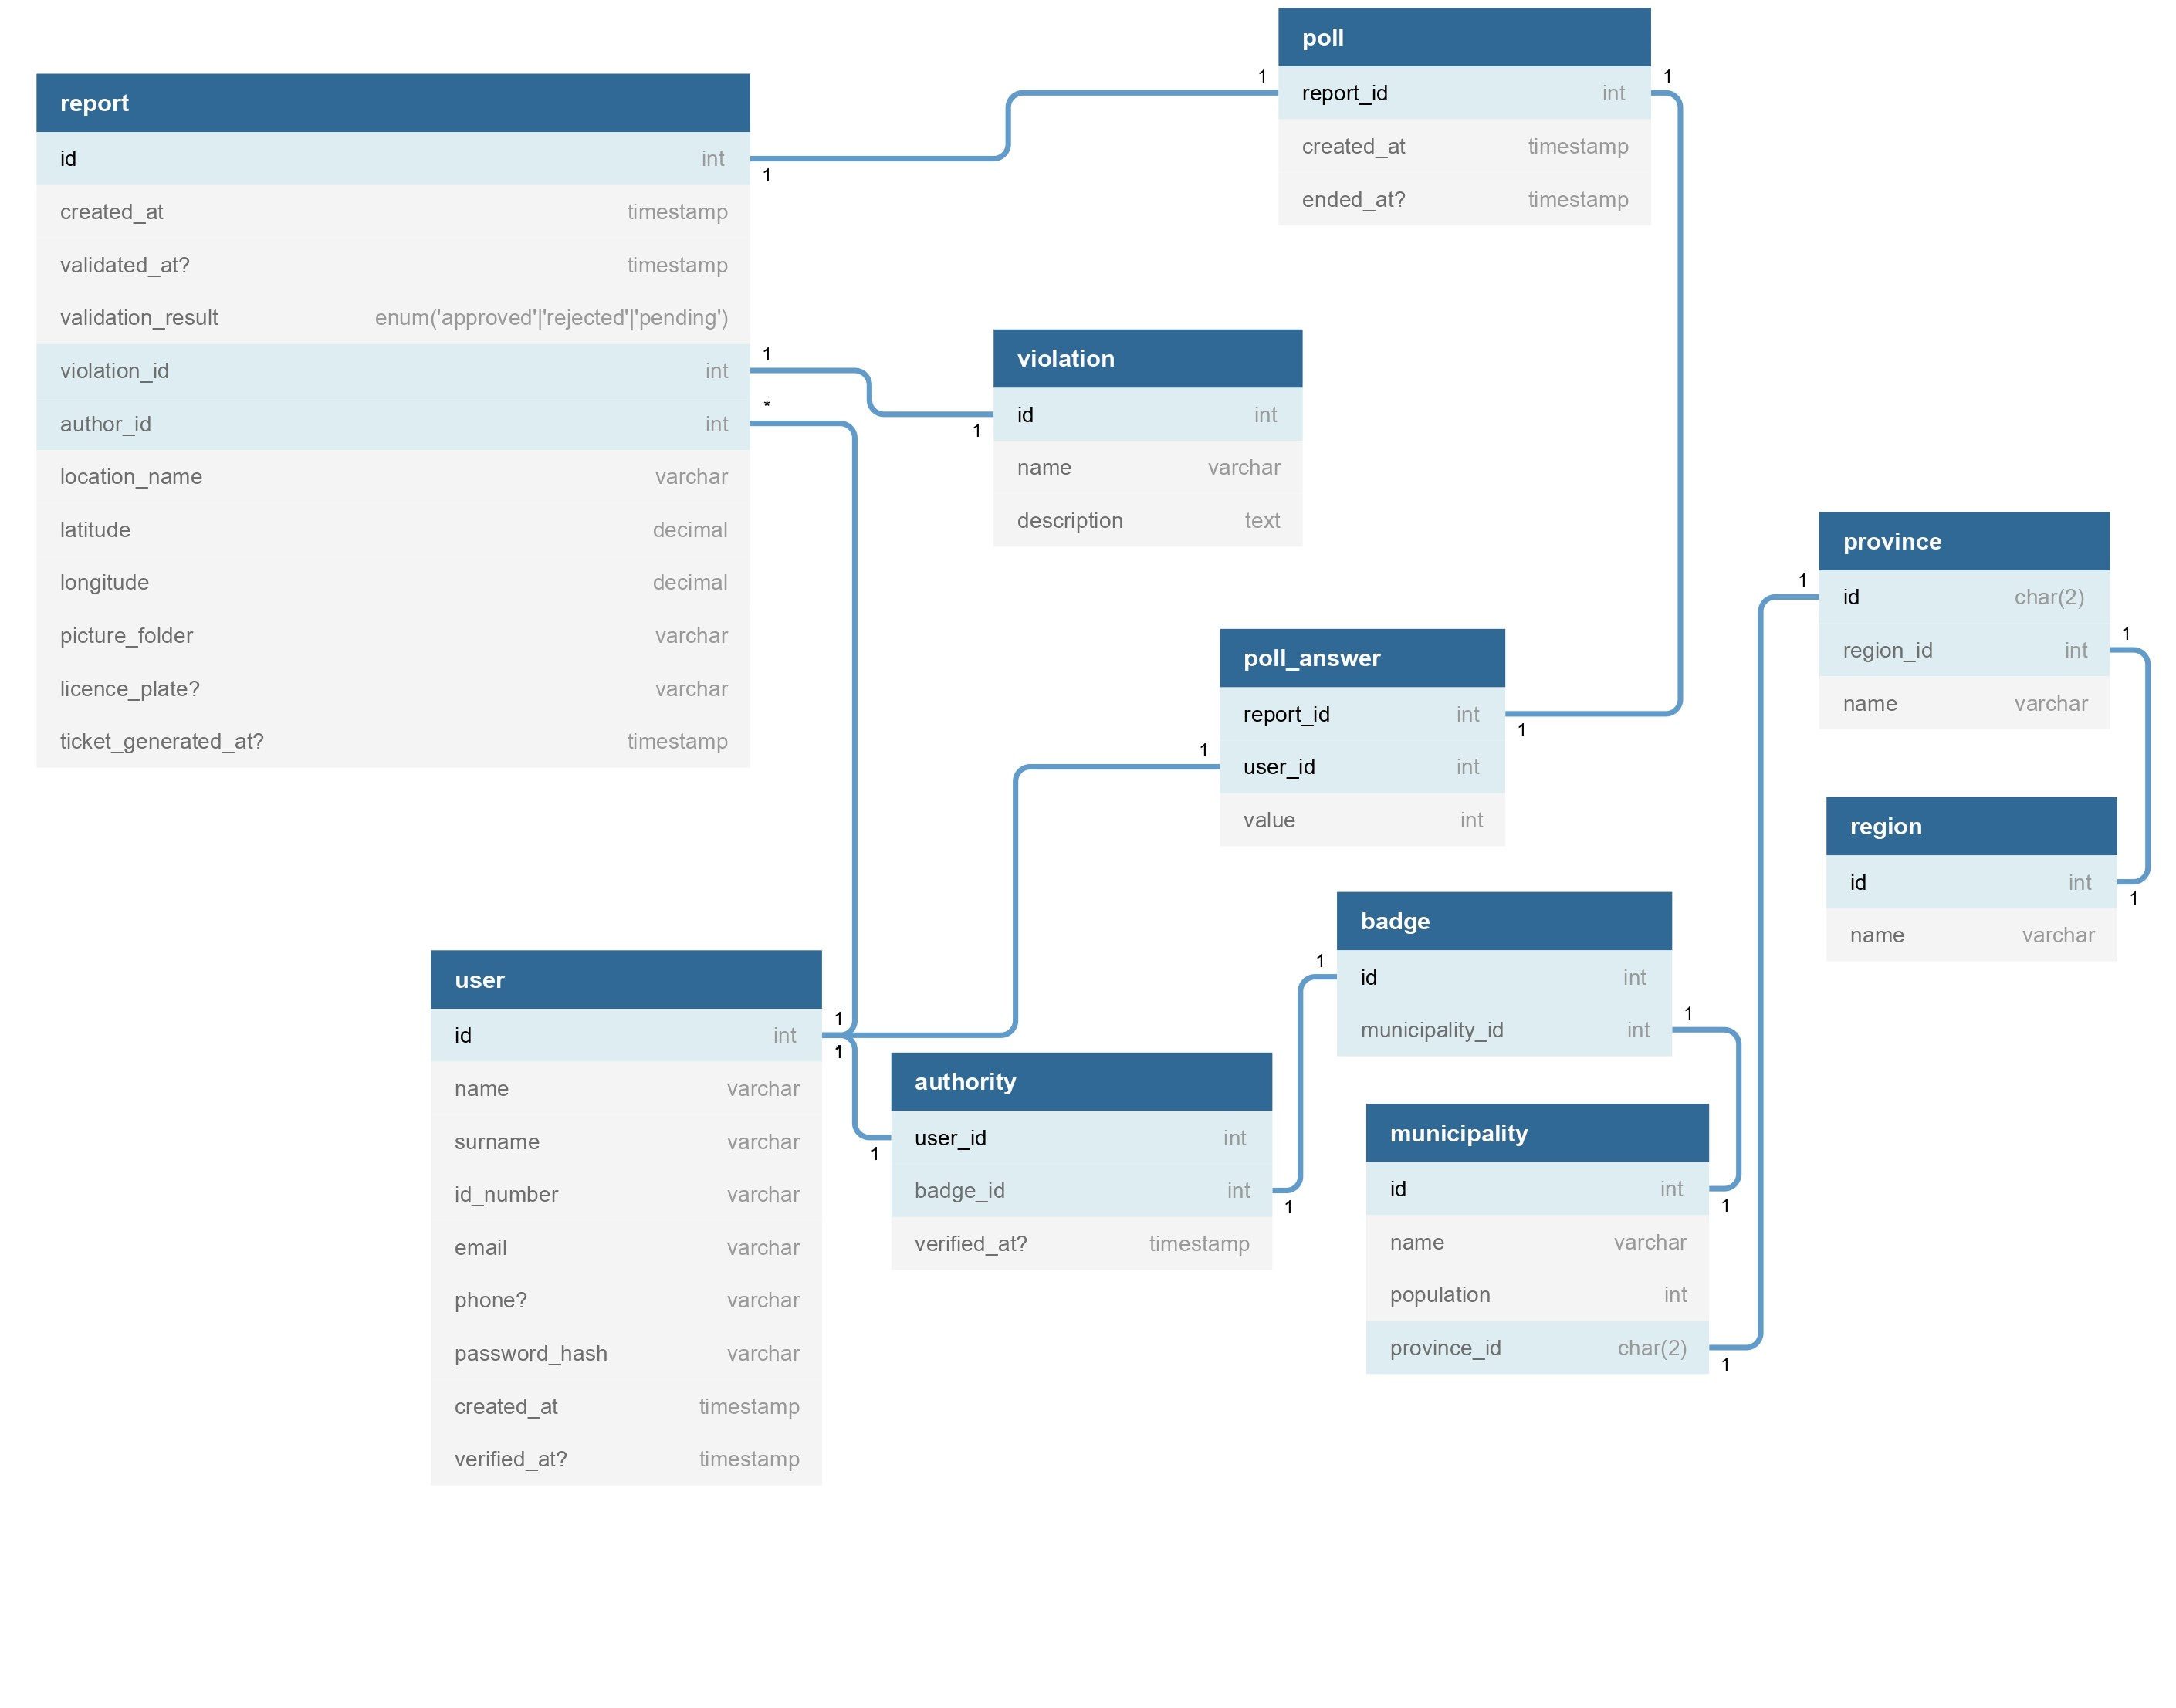
\includegraphics[origin=c,width=\textwidth]{DD_Images/RelationalModel/RelationalModel.jpg}
  \caption{\textit{Relational Model of RDBMS}}
\end{figure}

\subsubsection{Notes about Relational Model}
The diagram doesn't include fields that are obtainable with specific queries. An example is the score of a poll, that can be obtained 
with a view, or a materialized view. Another attribute, $validation\_result$, in Report entity, is 
inserted in the table, even if it could be computed with an inequality, because it is not granted that the threshold value will be constant 
in time. In fact, this value will depend on the number of active users that is monthly updated, or on other elements that make it 
variable.
\begin{itemize}
  \item \textit{"AttributeName?"} indicates an attribute that can assume NULL value. Most of the attributes are mandatory fields, only a few 
  can be nullable 
\end{itemize}

\subsection{Application Server}
This layer must handle a great part of the application logic, together with the connections with the data layer and the 
multiple ways of accessing the application from different clients. The main feature of the Application Server is the set 
of specific modules of logic, that describe rules regarding violations, their identification, and the following procedures. 
Work-flows for each of the functionalities provided by the application itself are also provided in this component. 
\newline The interface with the data layer must be handled by a dedicated persistent unit, that will be dedicated also to 
the dynamic data access and management, besides the object-relation mapping. In this way only the Application Server is 
granted to have access to the database.
\newline The Application Server must also provide a way to communicate with external systems, by adapting the application 
to already existing external infrastructures. 
\newline The main logic must include:
\begin{itemize}
  \item \textbf{UserModule}: This module will manage, through AccountModule component, all the logic involved with 
  the user account, management, and operations like registration, login, and also profile customization and update, as 
  allowed to authority, that can register with special permission after they are authorized. Furthermore, the module 
  will deal with the generation and provision of user credentials, connected to the optional two-factors authentication, 
  that can be requested by the client. Besides, this module has to manage user accounts; it has to store all the data 
  related to user accounts in the RDBMS, all the data related to users and to show stored data in case of personal data requests.
  \item \textbf{StatisticsModule}: This module contains the logic used to locate violations and users; besides it deals with the 
  definition of the Unsafe Area boundaries.This module must provide useful data to the logic that is at service of the unit 
  that deals with  Authorities, since it can need localization information, in order to perform its task.
  \item \textbf{AuthorityModule}: This module contains all the logic that grant access to an authority to its specific functionality: 
  generation of traffic tickets and access to personal information and sensible data regarding offenders. Besides, 
  the module is also devoted to the fundamental task of keeping the chain of custody of a certain notification with 
  license plate, in order to preserve the integrity of information.
  \item \textbf{ReportModule}: This module provides the function of collecting all the reports, it doesn't depend on the validity
  of notification itself. The module is used principally as a general collector, that provides the logic to collect reports that are
  provided by the user in a correct form. The reports are then sent to the ReportValidationModule in order to validate or reject them. 
  \item \textbf{ReportValidationModule}: This module provides the logic behind the report of violations, with particular 
  focus on timing restrictions and on the confirmation of the report by other users. This module is also in charge 
  of detecting multiple reports of the same violation. This module is useful to filter the reports, validating or rejecting them.
  \item \textbf{LicensePlateModule}: This module includes the logic needed by other components to set the license plate 
  status. It must also be useful as an interface with the external communication with the municipality, as it forwards a 
  certified license plate, after it has been validated under the supervision of an authority.
  \item \textbf{SuggestionsModule}: This module implements the algorithm to automatically generate suggestions in response to the
  violations notified and validated by SafeStreets. It uses the validated report, and provides suggestion to be sent to Municipality,
  that is an external agent to the system.
  \item \textbf{PushNotification}: This module is used as a gateway from all the modules that need to interact by 
  sending an email or a push notification to the clients. Its task is managing the logic behind the email and push notification services.
  \item \textbf{APIrest}: This module is used as an interface for the client to communicate with server and to send
  general requests. This module holds the general request of the client providing him the correct service he asked for.
\end{itemize}

\begin{figure}[H]
  \centering
  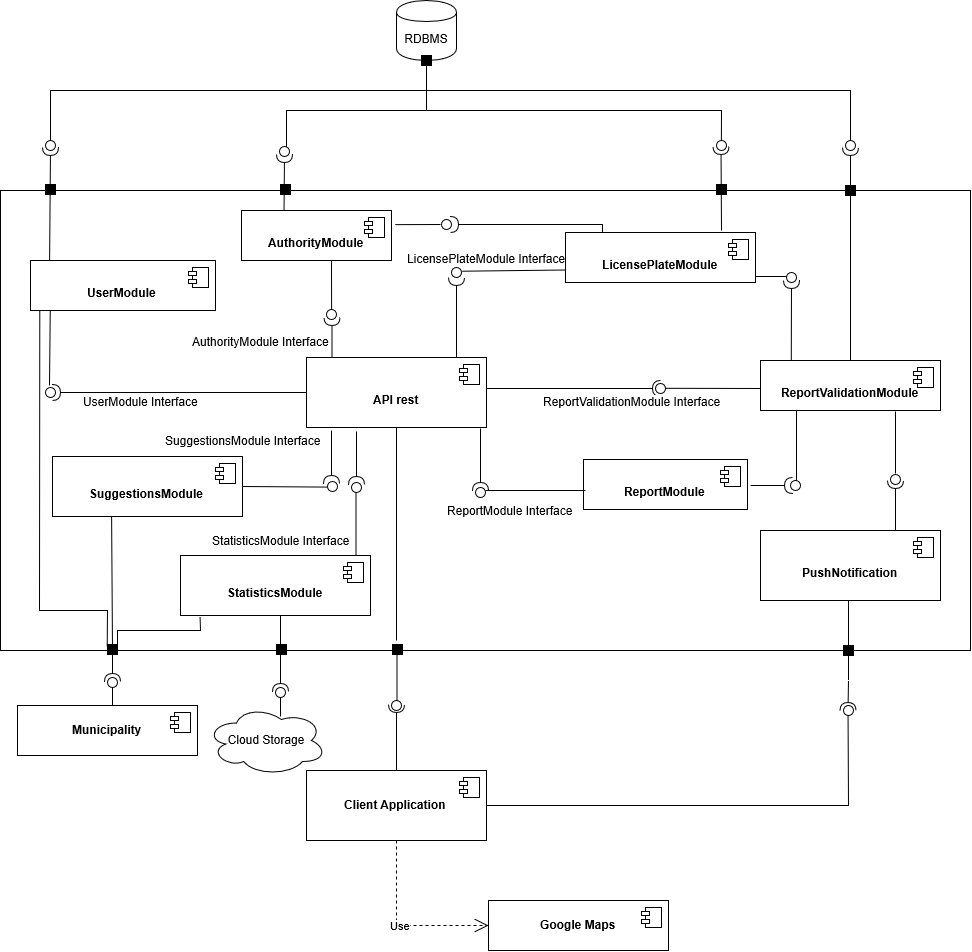
\includegraphics[origin=c,width=\textwidth]{DD_Images/ComponentView/componentViewServerZoom.jpg}
  \caption{\textit{Component View of the application - Focus on Application Server}}
\end{figure}

\begin{figure}[H]
  \centering
  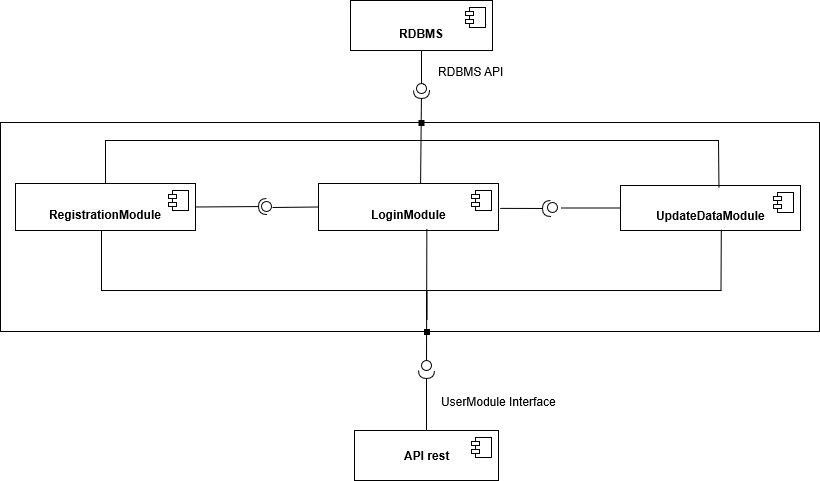
\includegraphics[origin=c,width=\textwidth]{DD_Images/ComponentView/componentViewUserModuleZoom.jpg}
  \caption{\textit{Component View of the application - Focus on UserModule of Application Server}}
\end{figure}

\subsection{Client Application}
The client must be designed in such a way to make the communication with the Application Server easy and not dependent 
on the implementation on both sides of communication. In order to reach this goal, adequate APIs must be defined and used 
to manage the interaction between the two components. The mobile application UI must be designed following the procedures 
provided by Android and iOS systems. The provided interface is suitable either for Mobile Client Application or Web Client Application,
as the client can connect to SafeStreets in both ways.
\newline The client application must provide a software module that manages GPS connection of the device and helps with 
the identification of location. This software will provide collected data to the Application Server to be processed. This 
is useful, but not fundamental for the application as the user is able to use SafeStreets also in absence of GPS 
functioning; in this case the location is manually inserted by the user.

